


\tikzset{every picture/.style={line width=0.75pt}} %set default line width to 0.75pt        

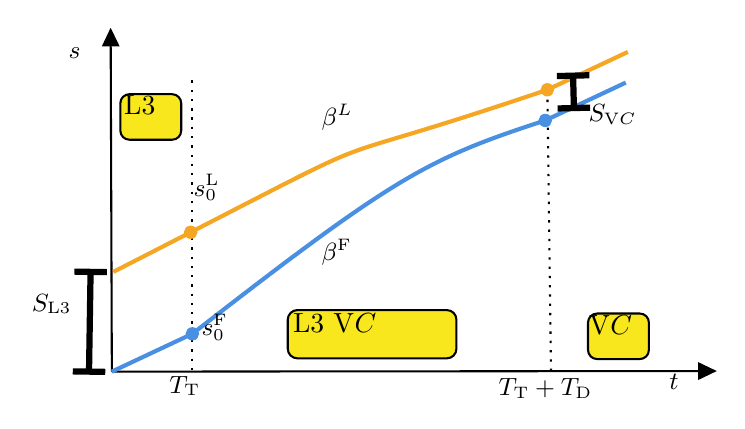
\begin{tikzpicture}[x=0.75pt,y=0.75pt,yscale=-1,xscale=1]
%uncomment if require: \path (0,300); %set diagram left start at 0, and has height of 300

%Straight Lines [id:da09966582141744862] 
\draw    (371.58,171.99) -- (660.03,171.71) ;
\draw [shift={(663.03,171.71)}, rotate = 179.94] [fill={rgb, 255:red, 0; green, 0; blue, 0 }  ][line width=0.08]  [draw opacity=0] (8.93,-4.29) -- (0,0) -- (8.93,4.29) -- cycle    ;
%Straight Lines [id:da6961264391561985] 
\draw    (371.58,171.99) -- (371.01,9.33) ;
\draw [shift={(371,6.33)}, rotate = 89.8] [fill={rgb, 255:red, 0; green, 0; blue, 0 }  ][line width=0.08]  [draw opacity=0] (8.93,-4.29) -- (0,0) -- (8.93,4.29) -- cycle    ;
%Curve Lines [id:da2265721045952236] 
\draw [color={rgb, 255:red, 245; green, 166; blue, 35 }  ,draw opacity=1 ][line width=1.5]    (409.56,104.85) .. controls (515.8,50.2) and (460.6,77.1) .. (581.4,36.2) ;
%Straight Lines [id:da9616751065584908] 
\draw [color={rgb, 255:red, 245; green, 166; blue, 35 }  ,draw opacity=1 ][line width=1.5]    (372.33,123.93) -- (409.56,104.85) ;
%Straight Lines [id:da018555734744043706] 
\draw [color={rgb, 255:red, 74; green, 144; blue, 226 }  ,draw opacity=1 ][line width=1.5]    (371.58,171.99) -- (410.36,153.77) ;
%Straight Lines [id:da9639137434101024] 
\draw  [dash pattern={on 0.84pt off 2.51pt}]  (410,31.67) -- (410,172.07) ;
%Shape: Ellipse [id:dp9112966542687357] 
\draw  [color={rgb, 255:red, 245; green, 166; blue, 35 }  ,draw opacity=1 ][fill={rgb, 255:red, 245; green, 166; blue, 35 }  ,fill opacity=1 ] (406.79,104.85) .. controls (406.79,103.36) and (408.03,102.15) .. (409.56,102.15) .. controls (411.08,102.15) and (412.32,103.36) .. (412.32,104.85) .. controls (412.32,106.34) and (411.08,107.55) .. (409.56,107.55) .. controls (408.03,107.55) and (406.79,106.34) .. (406.79,104.85) -- cycle ;
%Shape: Ellipse [id:dp29985741679191236] 
\draw  [color={rgb, 255:red, 74; green, 144; blue, 226 }  ,draw opacity=1 ][fill={rgb, 255:red, 74; green, 144; blue, 226 }  ,fill opacity=1 ] (407.6,153.77) .. controls (407.6,152.28) and (408.84,151.07) .. (410.36,151.07) .. controls (411.89,151.07) and (413.13,152.28) .. (413.13,153.77) .. controls (413.13,155.26) and (411.89,156.47) .. (410.36,156.47) .. controls (408.84,156.47) and (407.6,155.26) .. (407.6,153.77) -- cycle ;
%Straight Lines [id:da005349365428632069] 
\draw  [dash pattern={on 0.84pt off 2.51pt}]  (583.17,171.63) -- (581.4,36.2) ;
%Curve Lines [id:da29914220917049494] 
\draw [color={rgb, 255:red, 74; green, 144; blue, 226 }  ,draw opacity=1 ][line width=1.5]    (410.36,153.77) .. controls (508.6,77.4) and (523.8,69.4) .. (580.4,50.97) ;
%Shape: Ellipse [id:dp19607822283264786] 
\draw  [color={rgb, 255:red, 245; green, 166; blue, 35 }  ,draw opacity=1 ][fill={rgb, 255:red, 245; green, 166; blue, 35 }  ,fill opacity=1 ] (578.64,36.2) .. controls (578.64,34.71) and (579.87,33.5) .. (581.4,33.5) .. controls (582.93,33.5) and (584.16,34.71) .. (584.16,36.2) .. controls (584.16,37.69) and (582.93,38.9) .. (581.4,38.9) .. controls (579.87,38.9) and (578.64,37.69) .. (578.64,36.2) -- cycle ;
%Shape: Ellipse [id:dp14284725704573464] 
\draw  [color={rgb, 255:red, 74; green, 144; blue, 226 }  ,draw opacity=1 ][fill={rgb, 255:red, 74; green, 144; blue, 226 }  ,fill opacity=1 ] (577.64,50.97) .. controls (577.64,49.48) and (578.87,48.27) .. (580.4,48.27) .. controls (581.93,48.27) and (583.16,49.48) .. (583.16,50.97) .. controls (583.16,52.46) and (581.93,53.67) .. (580.4,53.67) .. controls (578.87,53.67) and (577.64,52.46) .. (577.64,50.97) -- cycle ;
%Straight Lines [id:da9229599929090104] 
\draw [color={rgb, 255:red, 74; green, 144; blue, 226 }  ,draw opacity=1 ][line width=1.5]    (580.4,50.97) -- (619.18,32.74) ;
%Straight Lines [id:da3997577781041448] 
\draw [color={rgb, 255:red, 245; green, 166; blue, 35 }  ,draw opacity=1 ][line width=1.5]    (581.4,36.2) -- (620.18,17.97) ;
%Straight Lines [id:da9429341700126102] 
\draw [line width=2.25]    (361.33,123.93) -- (360.58,171.99) ;
\draw [shift={(360.58,171.99)}, rotate = 270.89] [color={rgb, 255:red, 0; green, 0; blue, 0 }  ][line width=2.25]    (0,7.83) -- (0,-7.83)   ;
\draw [shift={(361.33,123.93)}, rotate = 270.89] [color={rgb, 255:red, 0; green, 0; blue, 0 }  ][line width=2.25]    (0,7.83) -- (0,-7.83)   ;
%Straight Lines [id:da5392239486107238] 
\draw [line width=2.25]    (593.8,29.4) -- (594.2,45) ;
\draw [shift={(594.2,45)}, rotate = 268.53] [color={rgb, 255:red, 0; green, 0; blue, 0 }  ][line width=2.25]    (0,7.83) -- (0,-7.83)   ;
\draw [shift={(593.8,29.4)}, rotate = 268.53] [color={rgb, 255:red, 0; green, 0; blue, 0 }  ][line width=2.25]    (0,7.83) -- (0,-7.83)   ;
%Rounded Rect [id:dp18201452495347814] 
\draw  [color={rgb, 255:red, 0; green, 0; blue, 0 }  ,draw opacity=1 ][fill={rgb, 255:red, 248; green, 231; blue, 28 }  ,fill opacity=1 ] (375.67,42.72) .. controls (375.67,40.3) and (377.63,38.33) .. (380.05,38.33) -- (400.61,38.33) .. controls (403.04,38.33) and (405,40.3) .. (405,42.72) -- (405,55.88) .. controls (405,58.3) and (403.04,60.26) .. (400.61,60.26) -- (380.05,60.26) .. controls (377.63,60.26) and (375.67,58.3) .. (375.67,55.88) -- cycle ;
%Rounded Rect [id:dp8291818582703099] 
\draw  [color={rgb, 255:red, 0; green, 0; blue, 0 }  ,draw opacity=1 ][fill={rgb, 255:red, 248; green, 231; blue, 28 }  ,fill opacity=1 ] (456.33,146.99) .. controls (456.33,144.42) and (458.42,142.33) .. (460.99,142.33) -- (532.95,142.33) .. controls (535.52,142.33) and (537.6,144.42) .. (537.6,146.99) -- (537.6,160.94) .. controls (537.6,163.51) and (535.52,165.6) .. (532.95,165.6) -- (460.99,165.6) .. controls (458.42,165.6) and (456.33,163.51) .. (456.33,160.94) -- cycle ;
%Rounded Rect [id:dp015062603676681219] 
\draw  [color={rgb, 255:red, 0; green, 0; blue, 0 }  ,draw opacity=1 ][fill={rgb, 255:red, 248; green, 231; blue, 28 }  ,fill opacity=1 ] (601,148.39) .. controls (601,145.96) and (602.96,144) .. (605.39,144) -- (625.95,144) .. controls (628.37,144) and (630.33,145.96) .. (630.33,148.39) -- (630.33,161.54) .. controls (630.33,163.97) and (628.37,165.93) .. (625.95,165.93) -- (605.39,165.93) .. controls (602.96,165.93) and (601,163.97) .. (601,161.54) -- cycle ;

% Text Node
\draw (349.28,14.53) node [anchor=north west][inner sep=0.75pt]  [font=\small]  {$s$};
% Text Node
\draw (638.74,171.79) node [anchor=north west][inner sep=0.75pt]  [font=\small]  {$t$};
% Text Node
\draw (409.51,75.49) node [anchor=north west][inner sep=0.75pt]  [font=\small]  {$s_{0}^{\mathrm{L}}$};
% Text Node
\draw (413.31,142.59) node [anchor=north west][inner sep=0.75pt]  [font=\small]  {$s_{0}^{\mathrm{F}}$};
% Text Node
\draw (471.11,106.49) node [anchor=north west][inner sep=0.75pt]  [font=\small]  {$\beta ^{\mathrm{F}}$};
% Text Node
\draw (331.53,133.13) node [anchor=north west][inner sep=0.75pt]  [font=\small]  {$S_{\mathrm{L} 3}{}$};
% Text Node
\draw (599.79,41.85) node [anchor=north west][inner sep=0.75pt]  [font=\small]  {$S_{\mathrm{V} C}{}$};
% Text Node
\draw (376.05,37.67) node [anchor=north west][inner sep=0.75pt]    {$\mathrm{L} 3$};
% Text Node
\draw (556.48,174.03) node [anchor=north west][inner sep=0.75pt]  [font=\small]  {$T_{\mathrm{T}} +T_{\mathrm{D}}$};
% Text Node
\draw (397.81,172.69) node [anchor=north west][inner sep=0.75pt]  [font=\small]  {$T_{\mathrm{T}}$};
% Text Node
\draw (457.39,142.33) node [anchor=north west][inner sep=0.75pt]    {$\mathrm{L} 3\ \leftrightarrows \mathrm{V} C$};
% Text Node
\draw (471.11,41.49) node [anchor=north west][inner sep=0.75pt]  [font=\small]  {$\beta ^{L}$};
% Text Node
\draw (600.05,143.33) node [anchor=north west][inner sep=0.75pt]    {$\mathrm{V} C$};


\end{tikzpicture}